\documentclass[11pt,a4paper]{article}
\ifdefined\pdfinfoomitdate\pdfinfoomitdate=1\fi
\ifdefined\pdftrailerid\pdftrailerid{}\fi
\ifdefined\pdfsuppressptexinfo\pdfsuppressptexinfo=15\fi
\usepackage[utf8]{inputenc}
\usepackage[T1]{fontenc}
\usepackage[spanish,es-nodecimaldot]{babel}
\usepackage{lmodern}
\usepackage{geometry}
\geometry{margin=2.2cm}
\usepackage{microtype}
\usepackage{amsmath,amssymb}
\usepackage{booktabs}
\usepackage{graphicx}
\usepackage{float}
\usepackage{xcolor}
\usepackage{hyperref}
\hypersetup{
  pdftitle={Reservorio fonónico de grafeno reducido: resultado negativo reproducible en simulación},
  pdfauthor={José Rodolfo Gómez Coeto},
  pdfsubject={Informe técnico de simulación reducida; sin validación experimental},
  colorlinks=true, linkcolor=blue!45!black, urlcolor=blue!55!black, citecolor=blue!45!black
}
\graphicspath{{../figures/}}
\newcommand{\TrialCount}{12}
\newcommand{\NarmaNonlinearMean}{1.033}
\newcommand{\NarmaLinearMean}{1.000}
\newcommand{\NarmaDelayMean}{0.502}
\newcommand{\NarmaNonlinearMinusLinear}{0.033}
\newcommand{\NarmaNonlinearMinusLinearLow}{0.018}
\newcommand{\NarmaNonlinearMinusLinearHigh}{0.048}
\newcommand{\NarmaNonlinearMinusDelay}{0.530}
\newcommand{\NarmaNonlinearMinusDelayLow}{0.504}
\newcommand{\NarmaNonlinearMinusDelayHigh}{0.556}
\newcommand{\ParityNonlinearMean}{0.497}
\newcommand{\ParityLinearMean}{0.501}
\newcommand{\ParityDelayMean}{0.502}
\newcommand{\ParityNonlinearMinusLinear}{-0.004}
\newcommand{\ParityNonlinearMinusLinearLow}{-0.014}
\newcommand{\ParityNonlinearMinusLinearHigh}{0.006}
\newcommand{\BootstrapSamples}{10000}
\newcommand{\NarmaNonlinearLow}{1.012}
\newcommand{\NarmaNonlinearHigh}{1.055}
\newcommand{\ParityNonlinearLow}{0.482}
\newcommand{\ParityNonlinearHigh}{0.513}
\newcommand{\MinimumAirGapFraction}{0.838}
\newcommand{\ContactThresholdFraction}{0.050}


\newcommand{\scopebox}[1]{\begin{center}\fcolorbox{black!35}{gray!7}{\parbox{0.92\linewidth}{#1}}\end{center}}

\title{Reservorio fonónico de grafeno reducido:\\resultado negativo reproducible en simulación}
\author{José Rodolfo Gómez Coeto}
\date{Versión 1.0.0 --- 14 de agosto de 2026}

\begin{document}
\maketitle

\begin{abstract}
Se auditó una propuesta de computación física basada en dinámica mecánica inspirada en resonadores de grafeno. El árbol original mezclaba simulación con afirmaciones de dispositivo, aplicaciones, costo y capacidad que no estaban sustentadas. Este informe limita el objeto a un modelo reducido, dependiente del hueco y consciente de contacto, y congela una comparación pareada de \TrialCount{} semillas. Bajo este protocolo, el modelo no lineal obtuvo NRMSE \NarmaNonlinearMean{} en NARMA-10, frente a \NarmaLinearMean{} de su ablación mecánica lineal y \NarmaDelayMean{} de una línea de retardo digital. En paridad-3 obtuvo exactitud \ParityNonlinearMean{}, indistinguible del azar. La evidencia, por tanto, \textbf{no apoya una ventaja computacional}. El aporte publicable es un resultado negativo reproducible y una delimitación explícita de lo que faltaría para estudiar un dispositivo real.
\end{abstract}

\scopebox{\textbf{Alcance.} Todo resultado de este documento proviene de simulación reducida. No hubo fabricación, medición, HIL, MCU, cuantización, FEM de una geometría concreta ni calibración óptica/electrónica. El protocolo no fue preregistrado externamente.}

\section{Pregunta y regla de decisión}
La hipótesis de trabajo era que una dinámica mecánica no lineal con lectura óptica podría proporcionar características útiles para tareas temporales, en línea con el marco general de reservoir computing físico \cite{tanaka2019,dion2018}. La pregunta comprobable se redujo a:

\begin{quote}
¿La condición mecánica no lineal supera, bajo semillas y readout pareados, a la misma dinámica linealizada y a una referencia digital de retardos en NARMA-10 o paridad-3?
\end{quote}

No se fijó una obligación de obtener un resultado positivo. Si la ventaja no aparecía, se detenían las afirmaciones de capacidad, aplicación y dispositivo. Esta regla evita ajustar selectivamente el relato a los gráficos producidos.

\section{Modelo reducido y dominio físico}
Se modelan $n=16$ modos/resonadores efectivos en un anillo periódico. No es una discretización espacial de una membrana y no representa fonones atomísticos. La ecuación por modo es
\begin{equation}
 m\ddot z_i=-m\omega_i^2z_i-\alpha_i z_i^3+k_c(z_{i-1}+z_{i+1}-2z_i)
 -m\gamma_i\dot z_i-\eta_i z_i^2\dot z_i+F_i(z_i,u).
\end{equation}
Resonadores de grafeno y amortiguamiento no lineal se han observado experimentalmente \cite{bunch2007,eichler2011}; esas referencias motivan la forma del modelo, pero no calibran estos parámetros. Para cada semilla se extraen 16 frecuencias de manera uniforme e independiente entre 10 y 40 MHz; las realizaciones exactas se serializan por trial en \texttt{results.json}.

La entrada modula el voltaje total $V_i=V_{dc}+V_{ac}w_i u$. Para un hueco de aire $g$ y óxido de espesor $d_{ox}$,
\begin{equation}
 F_i=\frac{\epsilon_0A}{2}\frac{V_i^2}
 {(g-z_i+d_{ox}/\epsilon_{ox})^2}.
\end{equation}
A diferencia de una fuerza constante, ésta crece al cerrarse el hueco. Si $g-z_i\leq0.05g$, el integrador falla con una excepción de contacto; no recorta la trayectoria y no extrapola a través del sustrato. Esto no constituye una predicción de \emph{pull-in}.

La lectura $x_i=R(g-z_i)-R(g)$ usa matriz de transferencia para capas de aire, grafeno, hueco, SiO$_2$ y Si. Se adopta $e^{-i\omega t}$ con índices pasivos $n=n_r+i\kappa$ y $\kappa\geq0$; la matriz de capa usa términos $-i\sin\delta$ y se contrasta en pruebas con una recursión de Fresnel independiente. Todos los modos comparten \textbf{un solo hueco nominal}; no se inventan puntos ópticos independientes. La interferometría Fabry--Pérot es pertinente para resonadores 2D \cite{aguila2022}, pero aquí los índices son ilustrativos y no una calibración experimental.

La ablación lineal fija $\alpha_i=\eta_i=0$ y conserva frecuencias, máscara, amortiguamiento, acoplamiento, electrostática y lectura óptica. Por eso aísla la no linealidad mecánica en este modelo, no toda fuente de no linealidad.

\section{Comprobaciones antes del benchmark}
La suite automatizada exige:
\begin{enumerate}
  \item reflectancia finita en $[0,1]$, periodicidad de $\lambda/2$ en la capa de aire y acuerdo con una recursión de Fresnel independiente para índices pasivos;
  \item fuerza electrostática creciente al reducir el hueco;
  \item fallo explícito al entrar en la región de contacto;
  \item disipación neta de energía sin excitación y con amortiguamiento positivo;
  \item acuerdo temporal entre pasos de $0.5$ y $0.25$ ns a periodo de símbolo fijo;
  \item repetibilidad con igual semilla y heterogeneidad distinta con semilla diferente;
  \item frecuencias y máscara idénticas entre condiciones pareadas.
\end{enumerate}
Estas pruebas verifican consistencia interna y convergencia temporal local, no FEM ni comparación con mediciones. En 48 trayectorias, el hueco mínimo fue $\MinimumAirGapFraction\,g$ frente al límite fail-closed de $\ContactThresholdFraction\,g$; ninguna rozó contacto.

\section{Protocolo estadístico}
Se congelan roles separados: semillas 4000--4011 para el modelo, 5000--5011 para NARMA-10 y 6000--6011 para paridad-3. Cada serie tiene 1200 símbolos; se descartan 200 y se divide cronológicamente el resto en 65\% de entrenamiento y 35\% de prueba. El escalado y los readouts sólo ven entrenamiento.

En regresión se ajustan \texttt{StandardScaler} y \texttt{Ridge} ($\alpha=10^{-3}$); en clasificación, \texttt{StandardScaler} y \texttt{RidgeClassifier} ($\alpha=1$). La referencia digital contiene 12 retardos. NARMA se evalúa con
\[
 \operatorname{NRMSE}=\sqrt{\mathbb E[(y-\hat y)^2]/\operatorname{Var}(y)}.
\]
Los intervalos son percentiles de \BootstrapSamples{} remuestras bootstrap de la media sobre los 12 pares. La semilla base es 20260814 y las diez subsemillas efectivas 20260814--20260823 se serializan por resumen en \texttt{results.json}. Son descriptores Monte Carlo del protocolo, no intervalos sobre dispositivos físicos. La literatura de capacidad de procesamiento \cite{dambre2012} no se usa para inferir una cota universal de este sistema.

\section{Resultado canónico}
\begin{table}[H]
\centering
\caption{Media sobre 12 pares. Menor NRMSE y mayor exactitud son mejores.}
\begin{tabular}{lrrr}
\toprule
Tarea & No lineal & Ablación lineal & Retardo digital\\
\midrule
NARMA-10, NRMSE & \NarmaNonlinearMean & \NarmaLinearMean & \NarmaDelayMean\\
Paridad-3, exactitud & \ParityNonlinearMean & \ParityLinearMean & \ParityDelayMean\\
\bottomrule
\end{tabular}
\end{table}

En NARMA-10, la diferencia pareada no lineal menos lineal fue $+\NarmaNonlinearMinusLinear$ con IC bootstrap 95\% $[+\NarmaNonlinearMinusLinearLow,+\NarmaNonlinearMinusLinearHigh]$. Como menor es mejor, la condición no lineal fue peor en esta parametrización. Frente al retardo digital, la diferencia fue $+\NarmaNonlinearMinusDelay$ $[+\NarmaNonlinearMinusDelayLow,+\NarmaNonlinearMinusDelayHigh]$.

\begin{figure}[H]
\centering
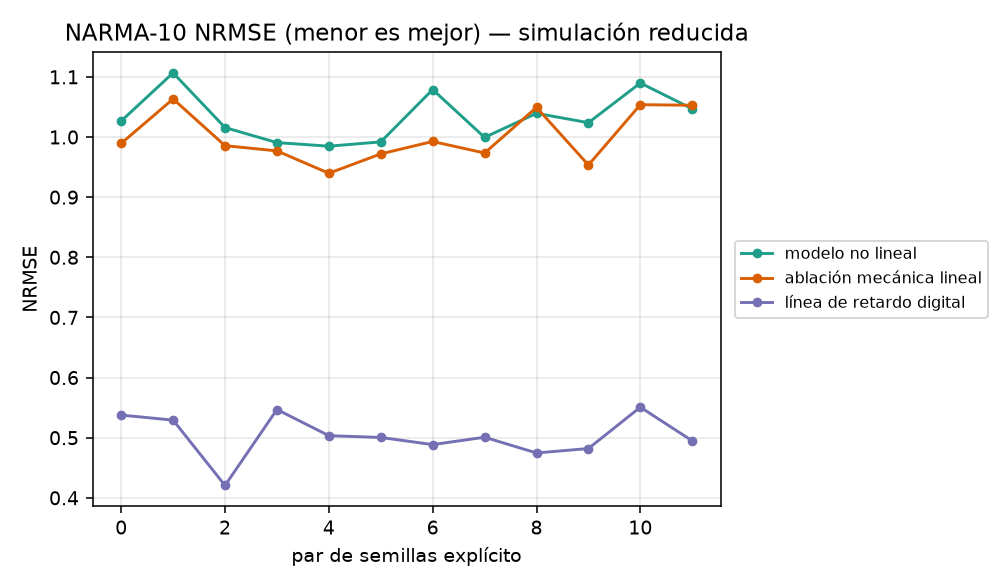
\includegraphics[width=0.82\linewidth]{paired_narma.png}
\caption{Resultado NARMA-10 por par de semillas. No se ocultan corridas adversas.}
\end{figure}

En paridad-3, la media no lineal fue \ParityNonlinearMean{} (IC de la media $[\ParityNonlinearLow,\ParityNonlinearHigh]$). La diferencia no lineal menos lineal fue \ParityNonlinearMinusLinear{} $[\ParityNonlinearMinusLinearLow,\ParityNonlinearMinusLinearHigh]$; el intervalo cruza cero y todos los promedios están cerca de 0.5.

\begin{figure}[H]
\centering
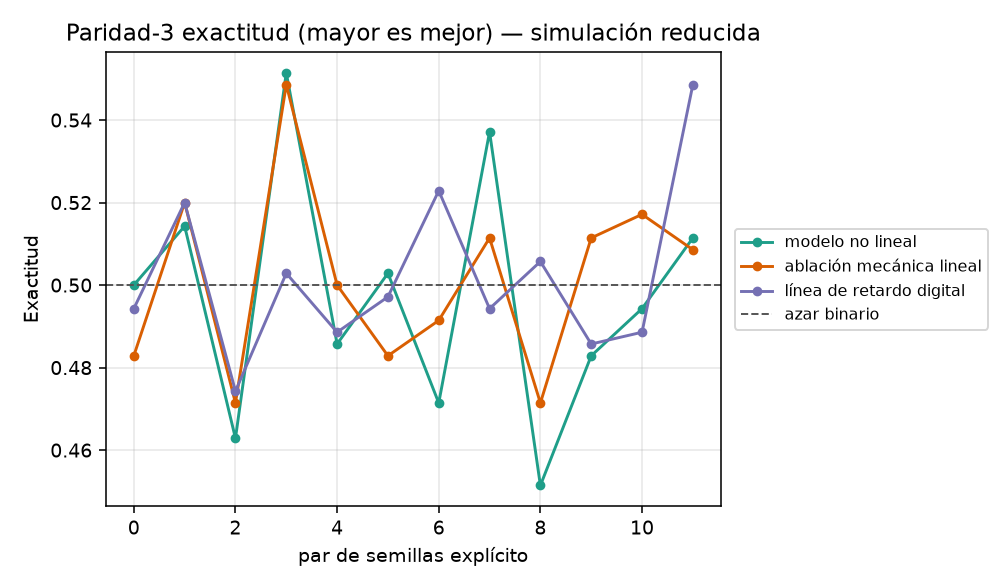
\includegraphics[width=0.82\linewidth]{paired_parity.png}
\caption{Exactitud de paridad-3; la línea discontinua marca azar binario.}
\end{figure}

\section{Interpretación y límites}
El resultado falsifica la afirmación concreta de ventaja bajo este punto operativo. No prueba que todo reservorio mecánico o de grafeno sea inútil; tampoco autoriza buscar retrospectivamente otra semilla o geometría y llamarla confirmación del mismo protocolo. Una variante futura sería un estudio nuevo.

Las causas posibles ---memoria insuficiente, observable poco informativo, punto operativo, readout o reducción modal--- no se identifican causalmente aquí. Ajustarlas después de observar estas métricas sería exploración, no validación.

Se retiraron del árbol público los benchmarks eléctricos/RF, dígitos, cuantización int8, costos de fabricación, potencia, comparación onda/difusión sesgada y proposiciones universales. La lista uno a uno está en \texttt{AUDIT\_RESOLUTION.md}.

\section{Qué falta para una hipótesis de dispositivo}
Antes de hablar de hardware serían necesarios, como mínimo: parámetros medidos de una geometría concreta; FEM/PDE convergente; curva de polarización y contacto; calibración interferométrica; arquitectura de excitación/adquisición; ruido, deriva y ancho de banda; y evaluación ciega con criterios fijados antes de observar resultados. Ninguno se infiere de la simulación actual.

\section{Reproducibilidad}
El entorno canónico fija Python 3.11.9 y dependencias transitivas. La entrada única
\begin{verbatim}
python -m pytest -q -p no:cacheprovider
python reproduce.py --compile-report
\end{verbatim}
regenera \texttt{results.json}, ambas figuras, las macros de esta tabla y el PDF. Los cinco payloads se producen fuera del árbol publicado. Bajo un lock de OS se sincroniza un journal durable antes del primer respaldo; si el proceso muere, la siguiente invocación restaura idempotentemente la generación anterior antes de generar. Se rechazan symlinks, junctions y reparse points en root, destinos, lock, backups y recovery. Un manifiesto estricto de tamaño/SHA-256 se instala al final. Las pruebas matan procesos después de cada backup y movimiento público, fuerzan rollback y unlock, y la suite vuelve a ejecutar las 12 parejas contra los artefactos congelados.

\section{Conclusión}
La auditoría no convirtió una idea especulativa en evidencia de dispositivo. Produjo algo más limitado pero verificable: un modelo reducido físicamente más coherente, un protocolo pareado sin fuga de prueba y un resultado negativo reproducible. En este protocolo, la no linealidad mecánica no aporta ventaja y no existe base para afirmar viabilidad de reservorio de grafeno.

{\small
\begin{thebibliography}{9}
\setlength{\itemsep}{0.15em}
\bibitem{tanaka2019} G. Tanaka et al., ``Recent advances in physical reservoir computing: A review,'' \emph{Neural Networks} 115, 100--123 (2019). \url{https://doi.org/10.1016/j.neunet.2019.03.005}
\bibitem{dion2018} G. Dion, A. Mejaouri y J. Sylvestre, ``Reservoir computing with a single delay-coupled non-linear mechanical oscillator,'' \emph{J. Appl. Phys.} 124, 152132 (2018). \url{https://doi.org/10.1063/1.5038038}
\bibitem{bunch2007} J. S. Bunch et al., ``Electromechanical Resonators from Graphene Sheets,'' \emph{Science} 315, 490--493 (2007). \url{https://doi.org/10.1126/science.1136836}
\bibitem{eichler2011} A. Eichler et al., ``Nonlinear damping in mechanical resonators made from carbon nanotubes and graphene,'' \emph{Nature Nanotechnology} 6, 339--342 (2011). \url{https://doi.org/10.1038/nnano.2011.71}
\bibitem{aguila2022} M. J. Aguila et al., ``Fabry--Pérot interferometric calibration of van der Waals material-based nanomechanical resonators,'' \emph{Nanoscale Advances} (2022). \url{https://doi.org/10.1039/D1NA00794G}
\bibitem{dambre2012} J. Dambre et al., ``Information Processing Capacity of Dynamical Systems,'' \emph{Scientific Reports} 2, 514 (2012). \url{https://doi.org/10.1038/srep00514}
\end{thebibliography}
}

\end{document}
